%%% ======= Beamer ======
\documentclass[usenames,dvipsnames,t]{beamer}
% \documentclass[usenames,dvipsnames, handout]{beamer}
\beamertemplatenavigationsymbolsempty % remove toolbar at the bottom of slides
\usepackage{appendixnumberbeamer} % for appendix
\usetheme{Madrid}
\usecolortheme{default}
\useinnertheme{circles}
\usepackage{soul}


\setbeamercolor{author in head/foot}{bg=blue!10, fg=blue}
\setbeamercolor{title in head/foot}{bg=blue!10, fg=blue}
\setbeamercolor{date in head/foot}{bg=blue!10, fg=blue}

\makeatletter
\setbeamertemplate{footline}{
  \leavevmode%
  \hbox{%
  \begin{beamercolorbox}[wd=.333333\paperwidth,ht=2.25ex,dp=1ex,center]{author in head/foot}%
    \usebeamerfont{author in head/foot}\insertshortauthor\expandafter\ifblank\expandafter{\beamer@shortinstitute}{}{~~(\insertshortinstitute)}
  \end{beamercolorbox}%
  \begin{beamercolorbox}[wd=.333333\paperwidth,ht=2.25ex,dp=1ex,center]{title in head/foot}%
    \usebeamerfont{title in head/foot}\insertshorttitle
  \end{beamercolorbox}%
  \begin{beamercolorbox}[wd=.333333\paperwidth,ht=2.25ex,dp=1ex,right]{date in head/foot}%
    \usebeamerfont{date in head/foot}\insertshortdate{}\hspace*{2em}
    \insertframenumber{}%
%     / \inserttotalframenumber
    \hspace*{2ex} 
  \end{beamercolorbox}}%
  \vskip0pt%
}
\makeatother

\colorlet{beamer@blendedblue}{blue!70} % change color theme


% For appendix
\newcommand{\backupbegin}{
   \newcounter{framenumberappendix}
   \setcounter{framenumberappendix}{\value{framenumber}}
}
\newcommand{\backupend}{
   \addtocounter{framenumberappendix}{-\value{framenumber}}
   \addtocounter{framenumber}{\value{framenumberappendix}} 
}

\setbeamertemplate{bibliography item}{\insertbiblabel} % improved references



% Other preamble stuff:
\usepackage{preamble}

%%% Uncomment for another color palette
% \definecolor{Logo1}{rgb}{0.0, 0, 0.7}
% \definecolor{Logo2}{rgb}{2.55, 2.55, 2.55}

% \setbeamercolor*{palette primary}{bg=Logo1, fg=white}
% \setbeamercolor*{palette secondary}{bg=Logo2, fg=white}
% \setbeamercolor*{palette tertiary}{bg=white, fg=Logo1}
% \setbeamercolor*{palette quaternary}{bg=white,fg=white}
% \setbeamercolor{structure}{fg=Logo1} % itemize, enumerate, etc
% \setbeamercolor{section in toc}{fg=Logo1} % TOC sections

% For figures
\usepackage{import}
\usepackage{xifthen}
\usepackage{pdfpages}
\usepackage{transparent}
\usepackage{mdframed}

% --- Inkscape figures:
\newcommand{\incfig}[2][0.75\textwidth]{%
    \def\svgwidth{\columnwidth}
    \resizebox{#1}{!}{\import{Inkscape figs/}{#2.pdf_tex}}
}

% --- Height of frame
\newlength{\myheight}
\setlength{\myheight}{7cm}


%------------------------------------------------------------
%This block of code defines the information to appear in the
%Title page
\title[\texttt{NMMA} long form] %optional
{\texttt{NMMA} long form update: \texttt{jax}}

\author{Thibeau Wouters}

\date{February 20, 2024}


%End of title page configuration block
%------------------------------------------------------------



%------------------------------------------------------------
%The next block of commands puts the table of contents at the 
%beginning of each section and highlights the current section:

\AtBeginSection[]
{
  \begin{frame}[plain, noframenumbering]
    \frametitle{Table of Contents}
    \tableofcontents[currentsection]
  \end{frame}
}

\AtBeginSubsection[]
{
  \begin{frame}[plain, noframenumbering]
    \frametitle{Table of Contents}
    \tableofcontents[currentsection]
  \end{frame}
}


%------------------------------------------------------------


\begin{document}

\begin{frame}[plain]
\titlepage
\end{frame}

% {

% \usebackgroundtemplate{\transparent{0.15}{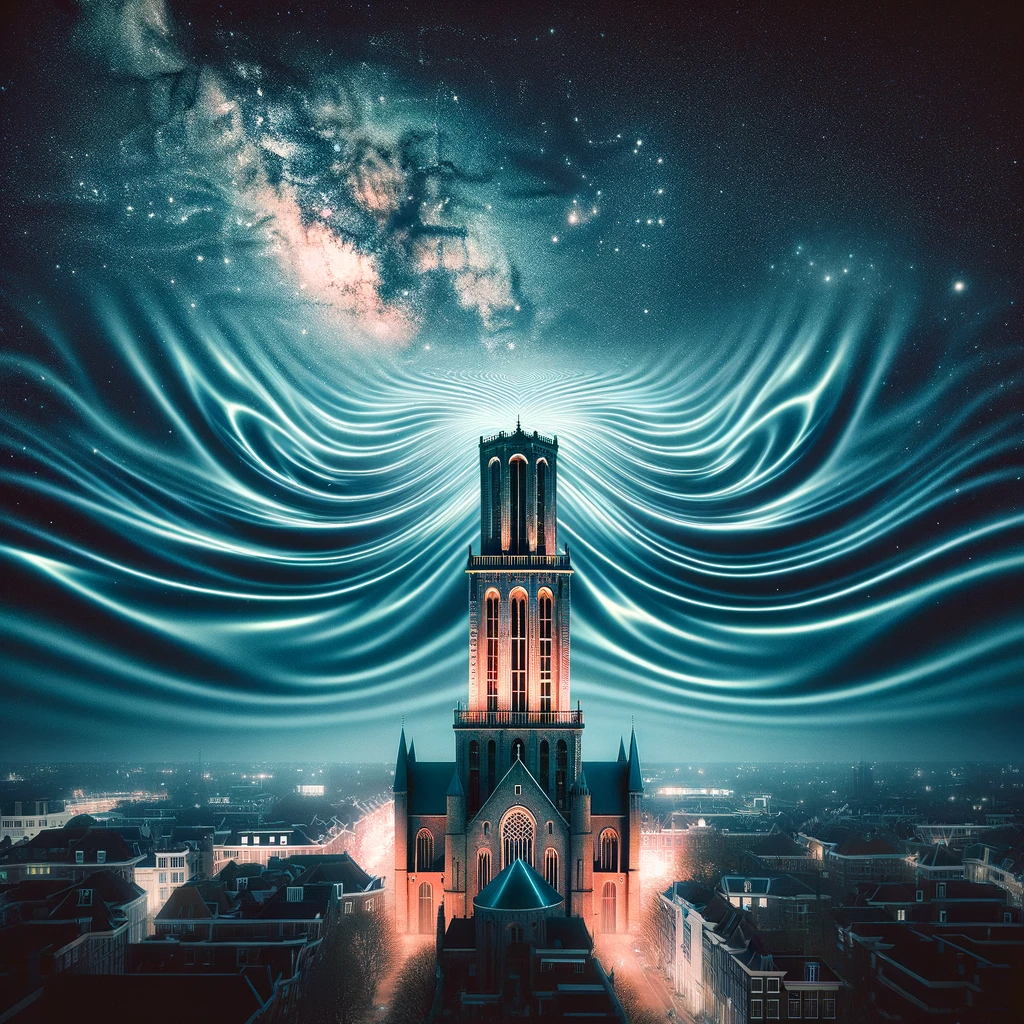
\includegraphics[width=\paperwidth,height=\paperheight]{Figures/ML4GWNL.png}}}

% \begin{frame}[plain]
% \titlepage

% \begin{figure}
% \centering
% 
\includegraphics[width=0.25\textwidth]{Figures/utrecht-university.png}
% \end{figure}

% \end{frame}
% }

% %The next statement creates the title page.
% \frame[plain]{\titlepage



% }


%---------------------------------------------------------
%This block of code is for the table of contents after
%the title page
\begin{frame}[plain, noframenumbering]
\frametitle{Table of Contents}
\tableofcontents
\end{frame}
%---------------------------------------------------------


\section{Introduction}

\begin{frame}{Parameter estimation}

\def\x{3mm}
\def\y{2mm}

\begin{itemize}
    \item Parameter estimation (PE): get \red{posterior} of GW/EM parameters $\theta$ % from data $d$
    \begin{equation*}
        \red{p(\theta | d)} = \frac{p(d | \theta) p(\theta)}{p(d)}
    \end{equation*}

    \vspace{\y}

    \item Sampling via Markov Chain Monte Carlo (MCMC)~\cite{brooks2011handbook}
    
    % \vspace{\y}
    
    % \item Computationally expensive
\end{itemize}

\vspace{\x}


\begin{tcolorbox}[colback=blue!10, boxrule=0pt]
  How to sample from high-dimensional, multi-modal posteriors?
\end{tcolorbox}

\vspace{2mm}

\centering
\incfig{MCMC_illustration}

\end{frame}

\begin{frame}{Overview}

  % % \def\x{2mm}

% We extend \texttt{jim} \cite{wong2023fast}, based on \texttt{jax} \cite{jax2018github}, with building blocks:
% \vspace{2mm}
% \begin{enumerate}
%   % \item 
  
%   % \vspace{\x}

%   \item Normalizing flow-enhanced, gradient-based MCMC (\texttt{flowMC}, \cite{gabrie2021efficient, wong2022flowmc})
  
%   \vspace{\x}

%   \item Automatically-differentiable (AD) GW (\texttt{ripple} \cite{edwards2023ripple})
  
%   \vspace{\x}

%   \item \gray{Relative binning likelihood \cite{zackay2018relative}}
% \end{enumerate}

% \vspace{-3mm}

% \incfig[\textwidth]{jim_flowMC_ripple}
  \def\x{2mm}

\begin{enumerate}
  \item \texttt{jax}~\cite{jax2018github}
  
  \vspace{\x}

  \item \texttt{flowMC}: Normalizing flow-enhanced, gradient-based MCMC~\cite{gabrie2021efficient, wong2022flowmc}
  
  \vspace{\x}

  \item \texttt{ripple}: Automatically-differentiable (AD) GW~\cite{edwards2023ripple}
  
  \vspace{\x}

  \item \texttt{jim}: Accelerated PE for GW~\cite{wong2023fast}
\end{enumerate}

\vspace{-3mm}

\incfig[\textwidth]{jim_flowMC_ripple}
  
\end{frame}

\section{Why \texttt{jax}?}

\begin{frame}{Why \texttt{jax}?}

  \def\x{4mm}

  \begin{tcolorbox}[colback=blue!10, boxrule=0pt]
    What are the benefits of \texttt{jax} for MCMC?
  \end{tcolorbox}

\vspace{3mm}

\begin{columns}
  \column{0.75\textwidth}
  \begin{enumerate}
    \item Automatic differentiation (AD)
    
    \vspace{\x}

    \item Just-in-time (JIT) compilation
    
    \vspace{\x}
    
    \item GPU acceleration
    
    \vspace{\x}
    
    \item Parallelization
    
    % \vspace{\x}
    
    % \item Vectorization
    
    % \vspace{\x}
    
    % \item Interoperability with \texttt{numpy}
  \end{enumerate}
  \column{0.20\textwidth}
  \begin{figure}
    % \centering
    
\includegraphics[width=\textwidth]{Figures/jax.png}
  \end{figure}
\end{columns}
  
\end{frame}

\section{\texttt{flowMC}}

\begin{frame}{\texttt{flowMC} -- local sampling}

\begin{enumerate}
  \item \textbf{Local sampling}: MALA (Metropolis-adjusted Langevin algorithm)
  
  \vspace{3mm}
  
  \begin{itemize}
    \item Proposal \red{$y$}: Langevin diffusion
    \begin{equation*}
      \red{y} = x + \frac{\epsilon^2}{2} \nabla \log p(x) + \epsilon \xi
    \end{equation*}

    \item Metropolis-Hastings acceptance step
  \end{itemize}
  
\end{enumerate}

\incfig[\textwidth]{MALA}

\end{frame}



\begin{frame}{\texttt{flowMC} -- normalizing flows}

\def\x{3mm}
\def\y{5mm}

Normalizing flows (NF):

\vspace{\x}

\begin{itemize}
  \item \blue{Latent space}: easy to sample (e.g. Gaussian)
  
  \vspace{\x}

  \item \red{Data space}: distribution learned from samples
  
  \vspace{\x}
  
  \item Enable approximate sampling from complicated distributions
\end{itemize}

\vspace{\y}
  
\incfig[\textwidth]{NF}

\end{frame}


\begin{frame}{\texttt{flowMC} -- global sampling}

  \def\x{3mm}
  \def\y{2mm}

  \begin{enumerate}
    \setcounter{enumi}{1}
    \item \textbf{Global sampling}
  \end{enumerate}

  \vspace{\x}

  \begin{itemize}
    \item Global proposal by sampling from NF
    
    \vspace{\y}
    
    \item Metropolis-Hastings acceptance step
  \end{itemize}

  \vspace{8mm}
  
  \incfig[\textwidth]{global_sampling}

\end{frame}



\begin{frame}{\texttt{flowMC} -- complete algorithm}

  \only<1>{\textbf{Training loop} \& Production loop}
  \only<2>{Training loop \& \textbf{Production loop}}

  \vspace{-5mm}  
  
  \only<1>{
    \incfig[\textwidth]{flowMC_loop}
  }

  \only<2>{
    \vspace{1cm}
    \incfig[\textwidth]{flowMC_loop_production}
  }

\end{frame}


\section{Results}

\begin{frame}{Results -- GW}
  \def\x{2mm}
  \def\y{-3mm}


  % Tidal waveform models in \texttt{ripple}:
  \begin{itemize}
    \item Reproduced PE for GW170817 \& GW190425 with TaylorF2
    
    \vspace{\x}

    \item Wrapping up injection studies
    
    \vspace{\x}

    \item Runtime: \st{$30$ min -- $1$ hour} \ \ $\mathbf{(17.11 \pm 2.65)}$ \textbf{min} (34 runs)
    
    % \vspace{\x}

    % \item \textit{i.e.}, if fully occupying \texttt{CIT}, \texttt{CITpcdev12}, ($4\times$ A100 GPU, 80 GB), $pp$-plot in $\approx 6$ hours
    
    \vspace{\x}

    \item \textbf{Current work}: tuning robustness/performance
  \end{itemize}

  \vspace{\y}

  % \incfig[\textwidth]{jim_flowMC_ripple}
  \vspace{8mm}
  \begin{figure}[H]
    \centering
    % 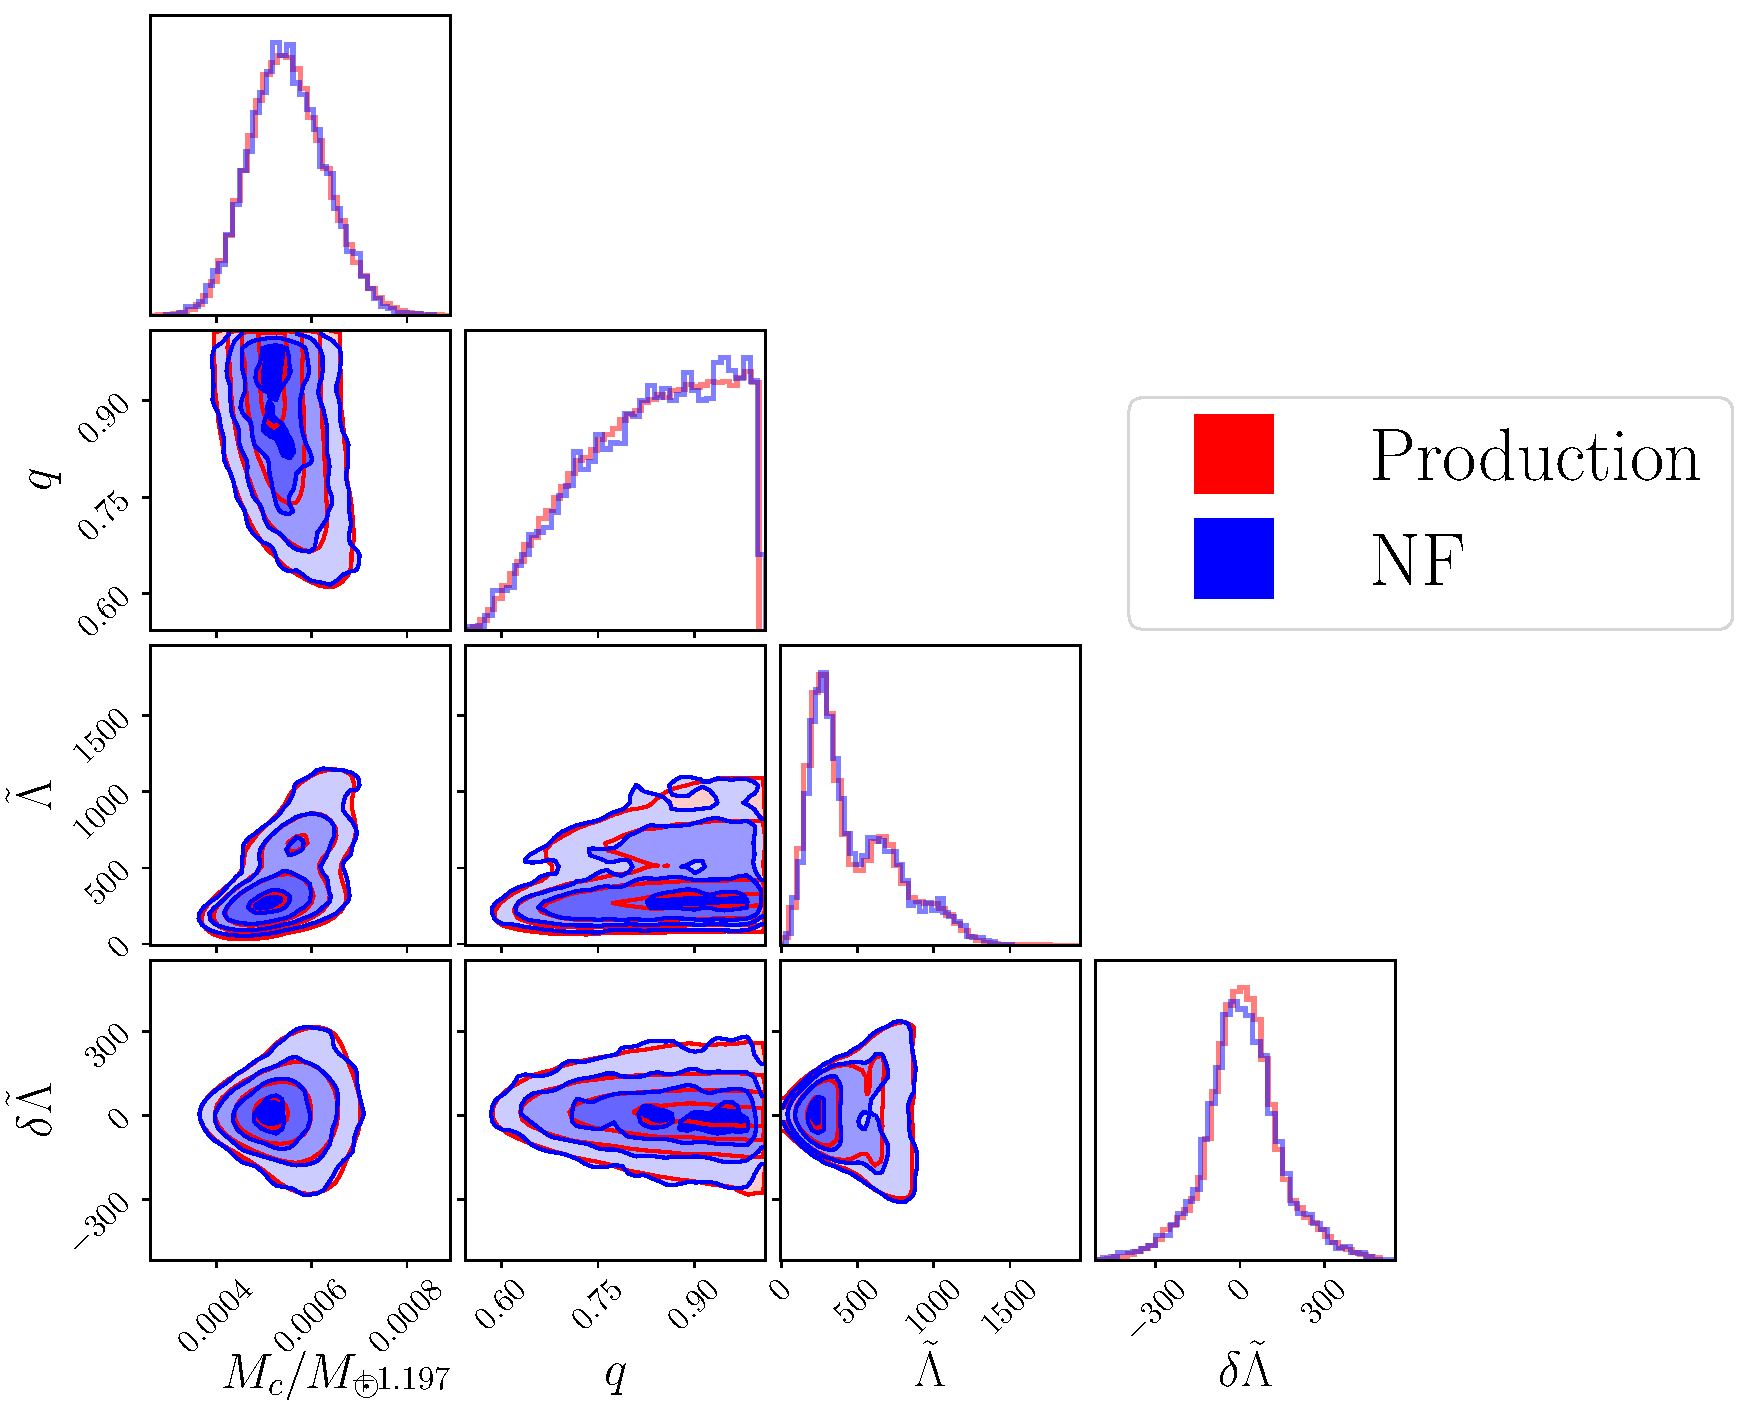
\includegraphics[scale=0.2]{Figures/presentation_GW170817_production_vs_NF_masses.pdf}
    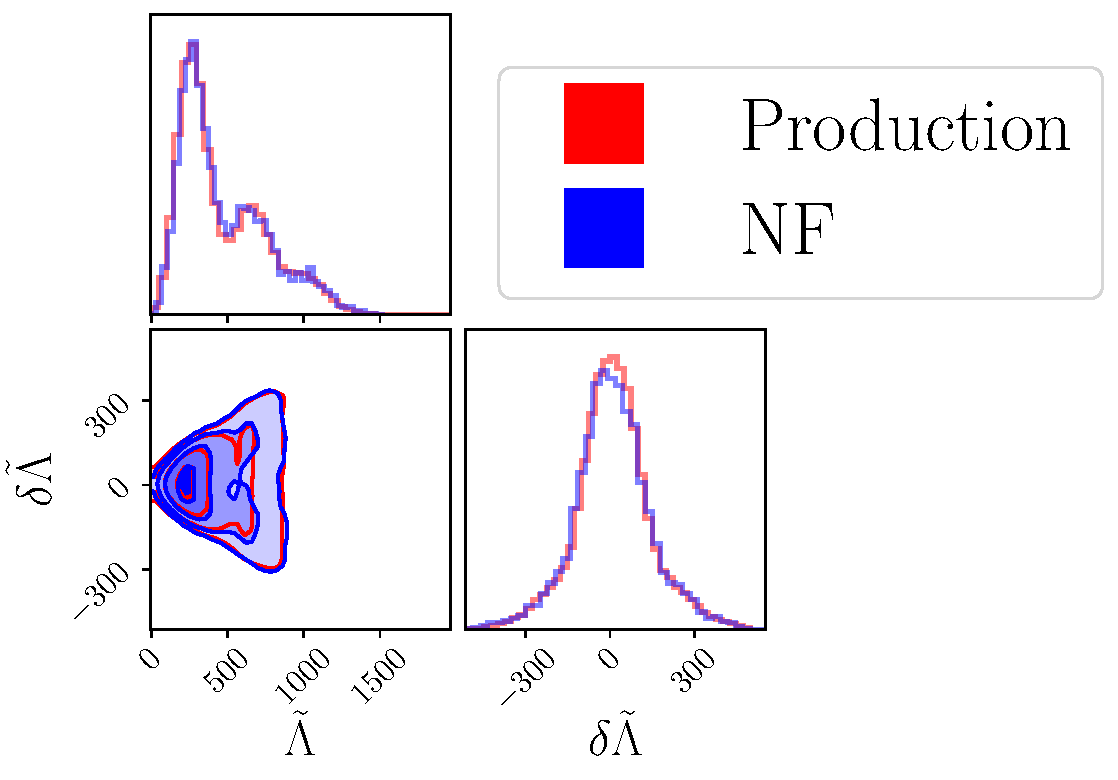
\includegraphics[width = 0.50\textwidth]{Figures/presentation_GW170817_production_vs_NF.pdf}
  \end{figure}
\end{frame}

\begin{frame}{Results -- EM}
  \def\x{4mm}


  % Tidal waveform models in \texttt{ripple}:
  \begin{itemize}
    \item Implemented surrogate model of Bu2022Ye with \texttt{flax}~\cite{flax2020github}
    
    \vspace{\x}

    \item Started on incorporating a \texttt{jax}-compatible likelihood for EM, but gives NaNs
    
    % \vspace{\x}

    % \item Cause? \texttt{jnp.where} with gradients? \href{https://jax.readthedocs.io/en/latest/faq.html\#gradients-contain-nan-where-using-where}{See the documentation}
    
    \vspace{\x}

    \item \textbf{Future work}: debug likelihood function, run first KN PE with \texttt{jax}
  \end{itemize}

\end{frame}


% \section{Future work \& conclusion}

% \begin{frame}{Future work}

%   \def\x{6mm}

%   \vspace{4mm}

%   \begin{itemize}
%     \item Finish IMRPhenomD\_NRTidalv2 in \texttt{ripple}
    
%     \vspace{\x}
    
%     \item Injection studies and pp-plot
    
%     \vspace{\x}

%     \item Update NF settings, boost efficiency
    
%     \vspace{\x}
    
%     \item Investigate synergy with simulation-based inference (\red{let's talk!})
    
%     % \vspace{\x}
    
%     % \item Investigate possibility of pretraining
%   \end{itemize}

% \end{frame}

% \begin{frame}{Conclusion}

%   \def\x{2mm}

%   \begin{itemize}
%     \item \texttt{flowMC}: NF-enhanced, gradient-based MCMC
    
%     \vspace{\x}
    
%     \item \texttt{ripple}: automatically differentiable GW
    
%     \vspace{\x}
    
%     \item $\texttt{jim} = \texttt{jax} + \texttt{flowMC} + \texttt{ripple}$
    
%     % \vspace{\x}
    
%     % \item \texttt{jim} is a promising tool for fast and accurate parameter estimation
    
%     \vspace{\x}

%     \item \texttt{jim} can do PE of BNS in $\sim 1$ min sampling/$\sim 30$ min wall time
    
%     \vspace{\x}
    
%     % \item \texttt{jim} can enhance and benefit from simulation-based inference
    
%   \end{itemize}

%   \vspace{-5mm}

%   \incfig[\textwidth]{jim_flowMC_ripple}
    
% \end{frame}

\section{Demo and homework}

\begin{frame}{Demo}

  \def\x{5mm}

  \begin{itemize}
    \item Time for a demo!
    
    \vspace{\x}

    \item Interested? Homework: check the Google docs
  \end{itemize}
      
\end{frame}

\begin{frame}[plain, noframenumbering]{References}

\printbibliography
    
\end{frame}

% ======== APPENDIX  ==========

\appendix

% \begin{frame}[plain, noframenumbering]

% \vfill

% \centering
% \textbf{BACK-UP SLIDES}

% \vfill

% \end{frame}


% \begin{frame}{Global acceptance for the NF}

%   \only<1>{
%     \begin{figure}
%       \centering
%       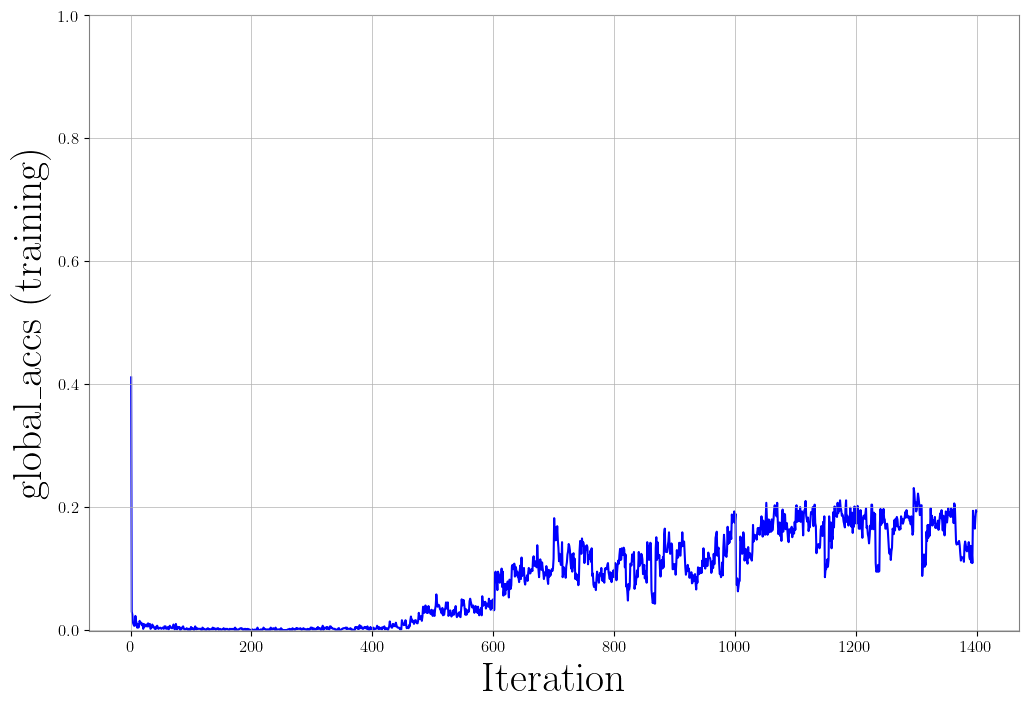
\includegraphics[width=0.8\textwidth]{Figures/global_accs_training.png}
%     \end{figure}  
%   }

%   \only<2>{
%     \begin{figure}
%       \centering
%       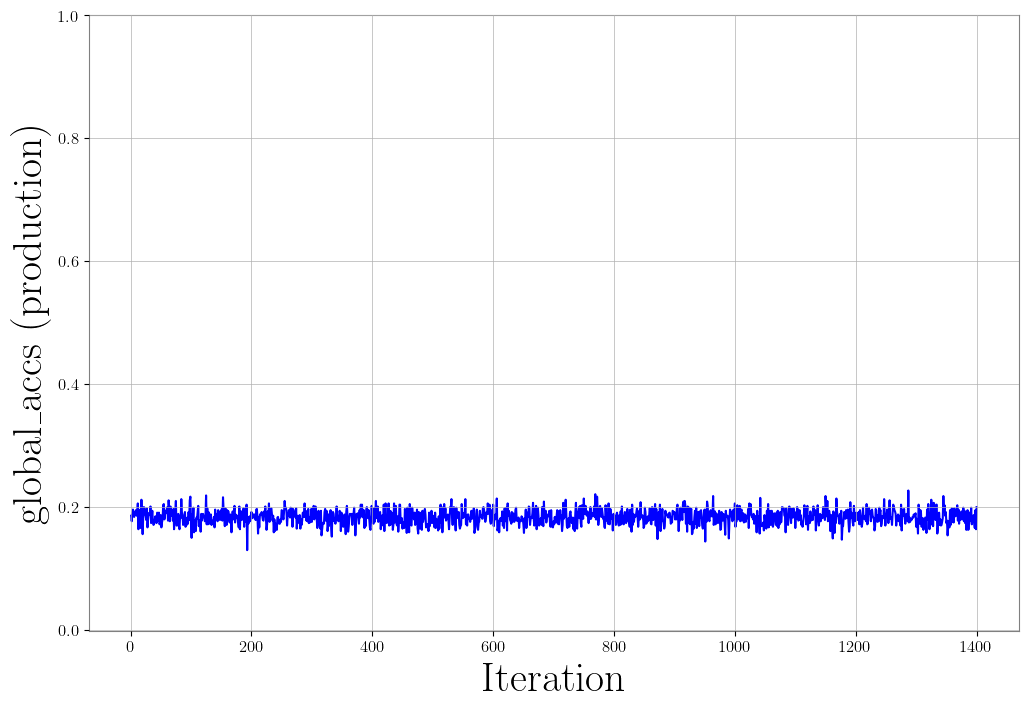
\includegraphics[width=0.8\textwidth]{Figures/global_accs_production.png}
%     \end{figure}  
%   }
  
% \end{frame}


% \begin{frame}{Full corner plot \href{https://ldas-jobs.ligo.caltech.edu/~thibeau.wouters/jim_runs/GW170817_TaylorF2/outdir/postprocessing_production_reweighted.png}{(link)}}

%   \begin{figure}
%     \centering
%     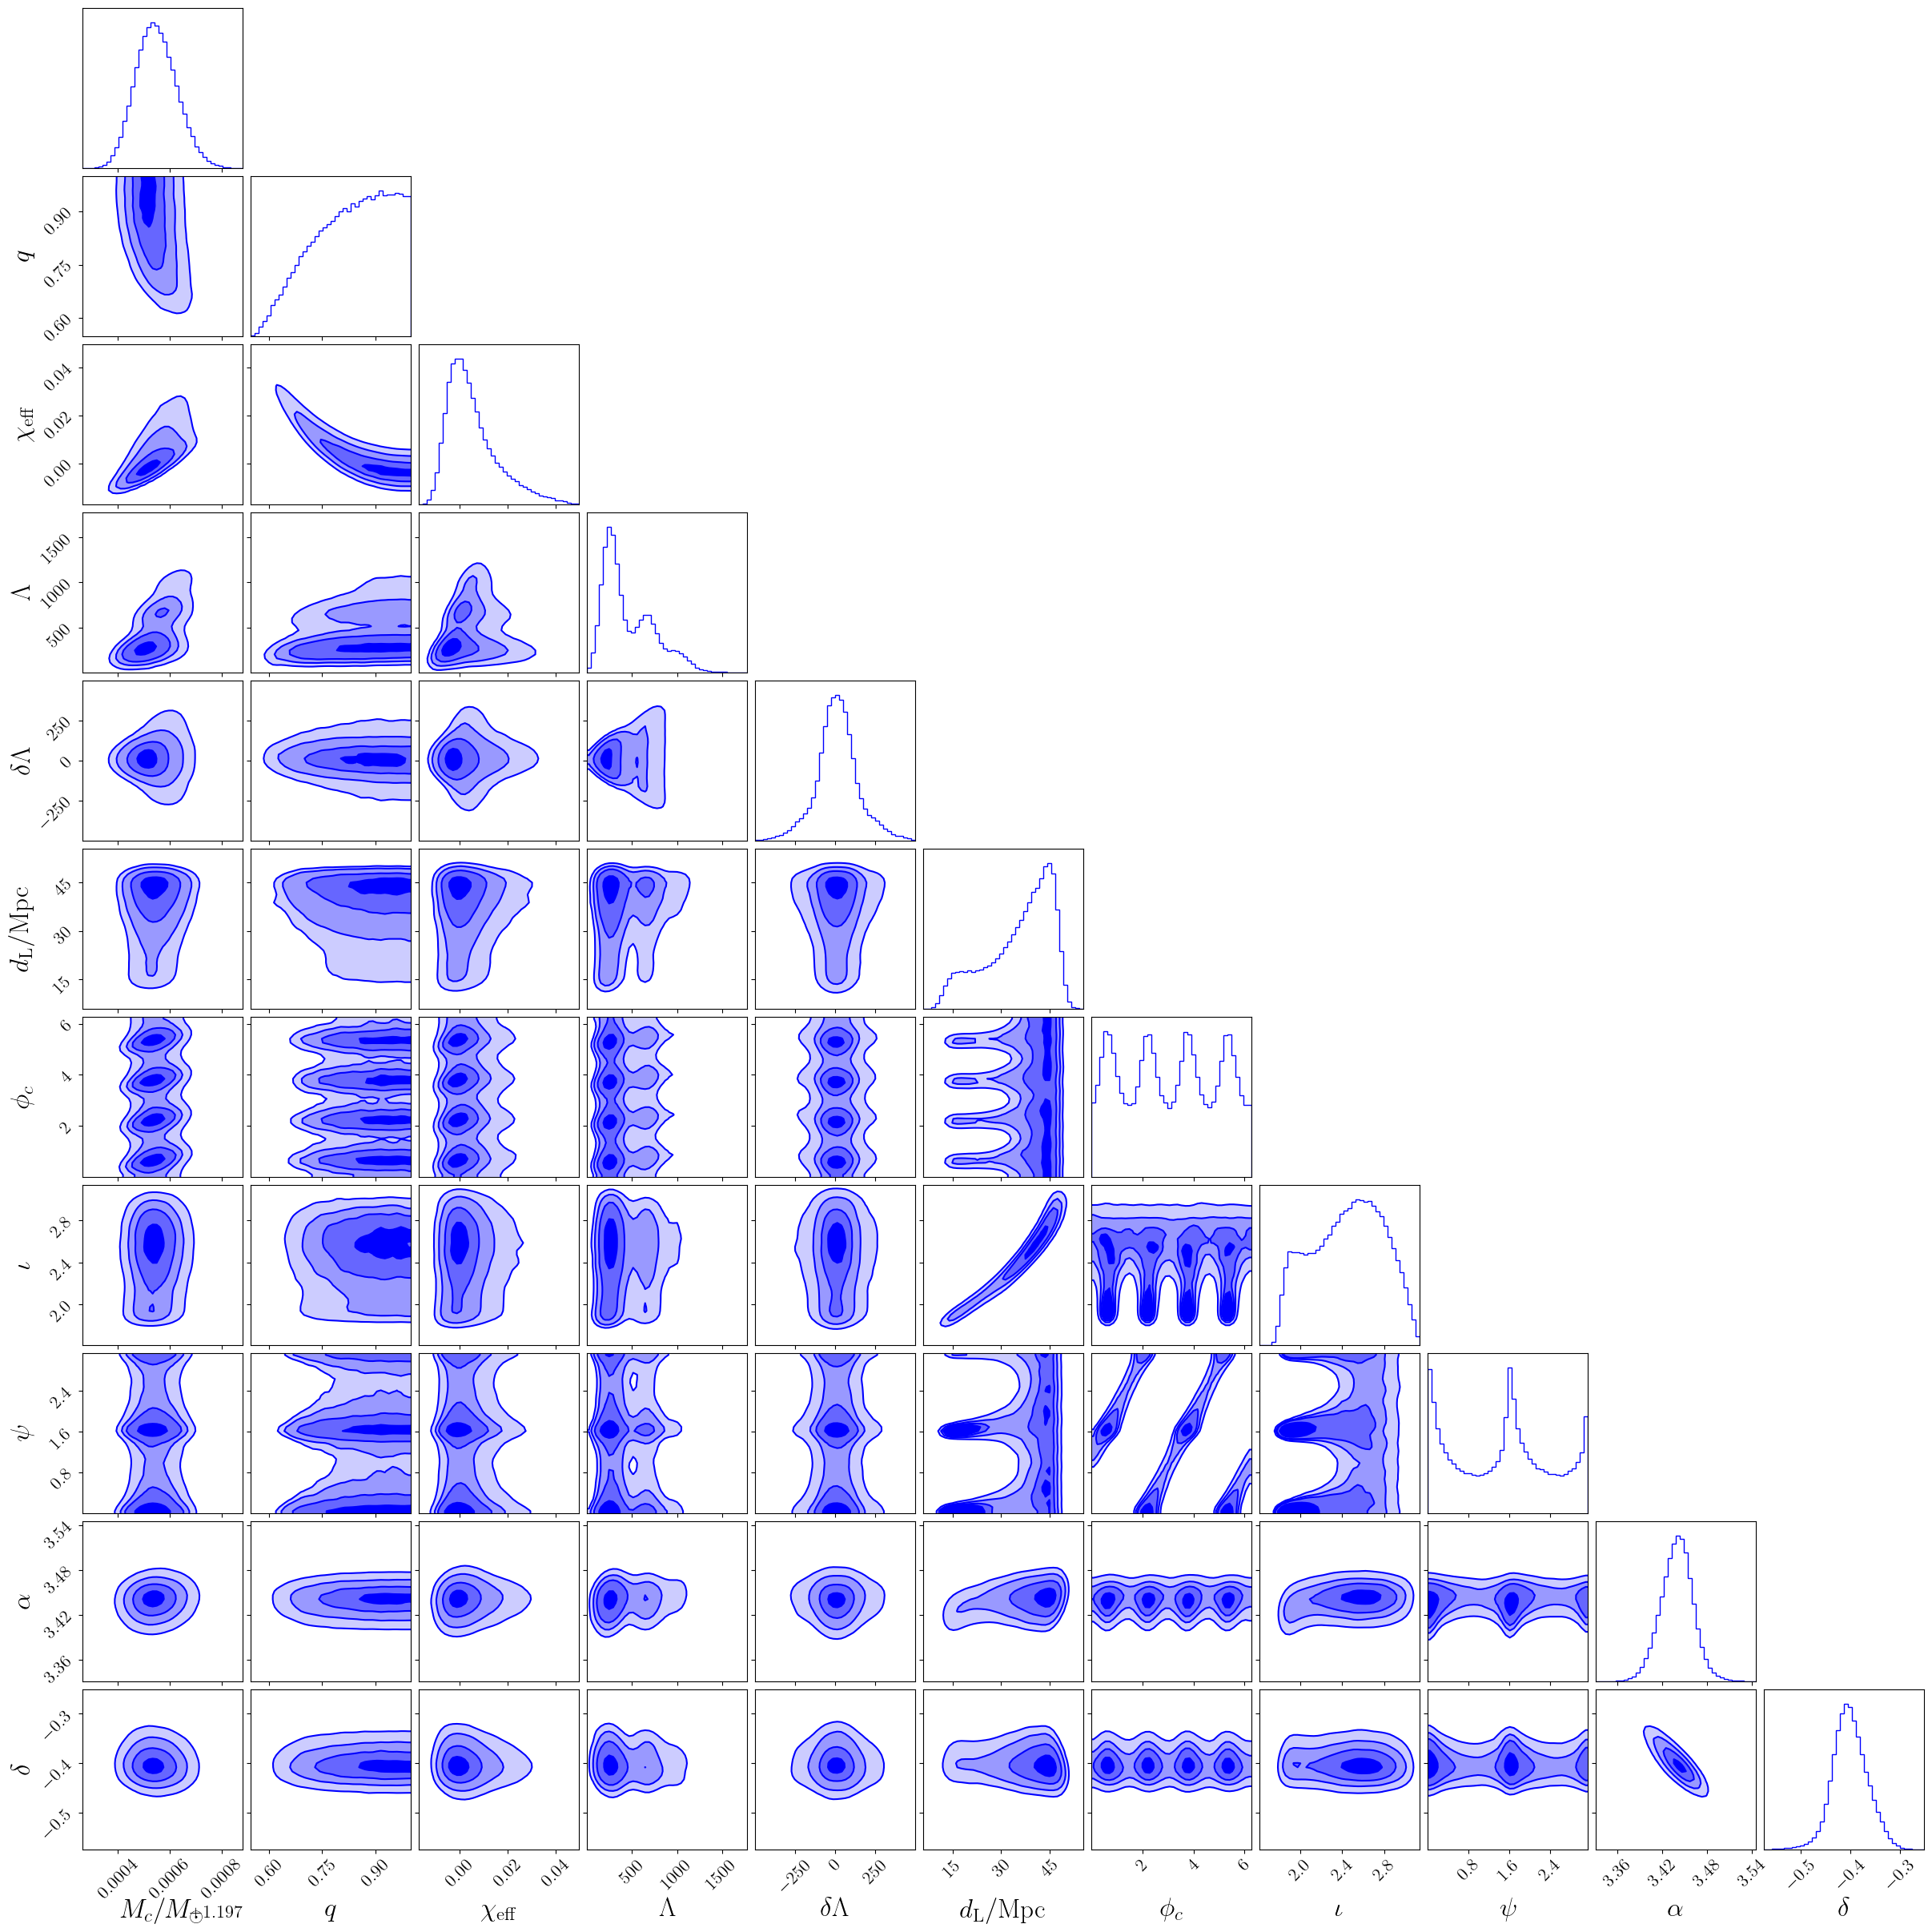
\includegraphics[scale=0.125]{Figures/full_corner.png}
%   \end{figure}  
% \end{frame}

\end{document}

